\documentclass[compress]{beamer}
%--------------------------------------------------------------------------
% Common packages
%--------------------------------------------------------------------------
%\usepackage[german]{babel}

% Figures
\usepackage{graphicx}
\graphicspath{{images/}}
\usepackage{subfig}

\usepackage{multicol}
% Erweiterte Tabellenfunktionen
\usepackage{tabularx,ragged2e}
\usepackage{booktabs}
% Listingserweiterung
\usepackage{listings}
\lstset{ %
language=[LaTeX]TeX,
basicstyle=\normalsize\ttfamily,
keywordstyle=,
numbers=left,
numberstyle=\tiny\ttfamily,
stepnumber=1,
showspaces=false,
showstringspaces=false,
showtabs=false,
breaklines=true,
frame=tb,
framerule=0.5pt,
tabsize=4,
framexleftmargin=0.5em,
framexrightmargin=0.5em,
xleftmargin=0.5em,
xrightmargin=0.5em
}

%--------------------------------------------------------------------------
% Load theme
%--------------------------------------------------------------------------
\usetheme{hsrm}

\usepackage{dtklogos} % must be loaded after theme
\usepackage{tikz}
\usetikzlibrary{mindmap,backgrounds}

%\usepackage[english]{babel}

\setbeamercovered{transparent=10}


\title{CodeCatch}
\subtitle{Extracting Source Code Snippets from Online Sources}
\author{Themistoklis Diamantopoulos\\ Georgios Karagiannopoulos\\ Andreas Symeonidis}
\institute{Electrical \& Computer Engineering Dept.\\ Aristotle University of Thessaloniki}

%\date{\today}

\begin{document}

\maketitle

\section*{Contents}
\begin{frame}
	\frametitle{CONTENTS}
	\tableofcontents[hideallsubsections]
\end{frame}

\section{Introduction}

\begin{frame}{Recommendation Systems}
\onslide<1->
The routine process of writing new code involves using search engines to find \lstinline!snippets! from websites like StackOverflow, blogs, documentation etc.

\vfill
This approach is time-consuming, distracting, and implies a lot of personal effort by the developer.

\onslide<2->
\vfill
{\Medium CodeCatch}: A system that accelerates the process of searching and separating the solutions for a specific programming task.


\end{frame}

\begin{frame}{Related Work}
\onslide<1->
Many similar systems have been proposed in the past:

\quoted {Prospector, PARSEWeb, MAPO, UP-Miner, PAM, APIMiner, eXoaDocs, DECKARD, Blueprint, ...}

\alert{Deficits} of the aforementioned systems:

\onslide<2->
\begin{itemize}
	\item Too much knowledge is required beforehand for the API to be used.
	\item Most of them do not return ready-to-use snippets.
	\item Results are presented in form of lists setting the different implementations difficult to separate.
	\item They preserve local indexes with limited size and diversity and sometimes outdated.
	\item Quality and reusability of results usally not evaluated.
	\item They involve some specialized query language requiring additional effort.
\end{itemize}

\end{frame}

\section{Zweite Sektion}
\begin{frame}{CodeCatch System Overview}

\begin{figure}
	\centering
	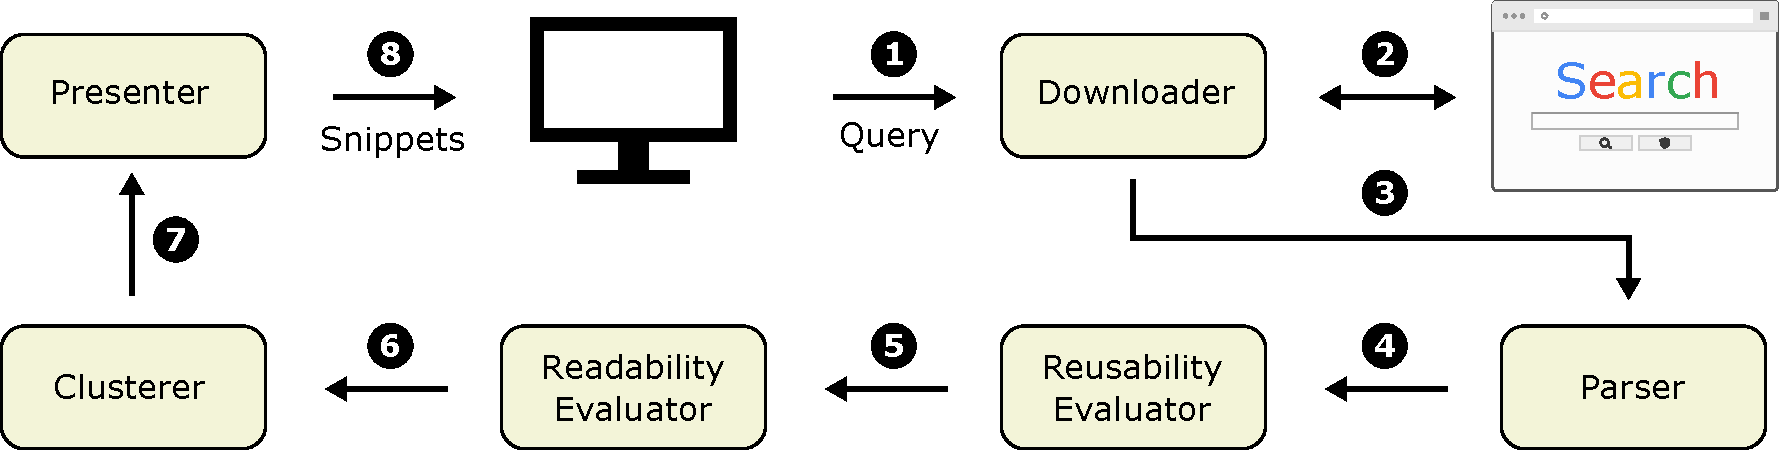
\includegraphics[width=\textwidth]{systemoverviewnew}
	\caption{The components of CodeCatch and how they are connected.}
\end{figure}

\end{frame}

\begin{frame}{Downloader}

\begin{figure}
	\centering
	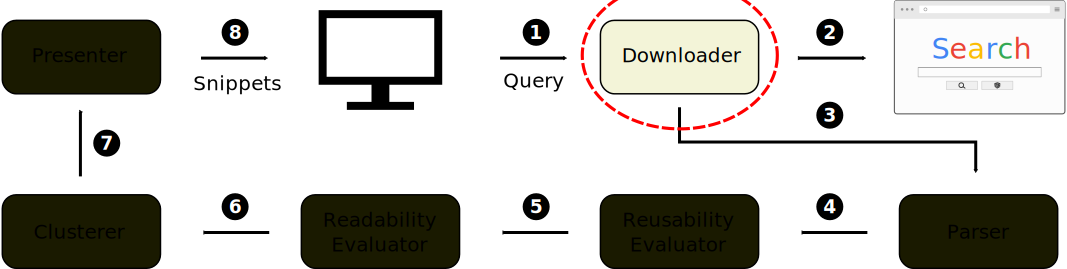
\includegraphics[width=\textwidth]{downloader}
\end{figure}

\end{frame}

\end{document}






